\documentclass[11pt,a4paper]{article}

\usepackage[margin=1in]{geometry}
\usepackage[T1]{fontenc}
\usepackage[utf8]{inputenc}
\usepackage{lmodern}
\usepackage{amsmath,amssymb}
\usepackage{booktabs}
\usepackage{array}
\usepackage{longtable}
\usepackage{caption}
\usepackage{enumitem}
\usepackage{hyperref}
\usepackage{tikz}
\usetikzlibrary{arrows.meta,calc,positioning}

\hypersetup{hidelinks}

\setlength{\parindent}{1.2em}
\setlength{\parskip}{0.25em}
\setlist[itemize]{topsep=0.3em,itemsep=0.15em}
\setlist[enumerate]{topsep=0.3em,itemsep=0.15em}

\newcolumntype{L}[1]{>{\raggedright\arraybackslash}p{#1}}
\newcommand{\sectionpage}{\clearpage}

\title{\textbf{Modeling and Control of an Underactuated Cart Double-Pendulum in MATLAB}}
\author{Your Name}
\date{4 May 2026}

\begin{document}
\maketitle

\begin{abstract}
This paper presents a MATLAB implementation of an underactuated cart with a serial double pendulum. The plant has three generalized coordinates and a single control input, making it a representative nonlinear benchmark for robotics and control. The model is derived in Euler--Lagrange form and implemented as a state-space function suitable for numerical integration with \texttt{ode45}. The implementation includes model verification by energy conservation, equilibrium checks, numerical and analytic linearization, and controllability analysis. Two control approaches are then considered. The first is a local linear quadratic regulator (LQR) designed around the upright equilibrium. The second is a nonlinear energy-shaping swing-up controller with a switching law that transfers control to the local LQR near the upright configuration. The report discusses the structure, assumptions, controller logic, and expected simulation behavior of the MATLAB project.
\end{abstract}

\noindent\textbf{Keywords:} underactuated robotics, Euler--Lagrange modeling, cart-pendulum, LQR, energy shaping, MATLAB simulation.

\sectionpage
\section{Introduction}

Underactuated mechanical systems are systems with fewer independent actuators than degrees of freedom. They appear frequently in robotics, aerospace systems, legged locomotion, pendulum benchmarks, and flexible mechanical structures. Their behavior is challenging because not every coordinate can be directly commanded. Instead, the controller must exploit the natural coupling between actuated and unactuated coordinates. This makes underactuated systems useful for studying nonlinear dynamics, model-based control, and the limitations of local linear methods.

The MATLAB project considered in this paper studies a cart with a serial double pendulum. The cart can move horizontally and is actuated by a single horizontal force. The two pendulum links are passive, so the controller has to influence their motion indirectly through cart acceleration. The full system has three generalized coordinates: the cart position $s$, the first pendulum angle $\theta_1$, and the second pendulum angle $\theta_2$. Since only the cart coordinate is actuated, the system has three mechanical degrees of freedom but only one input.

The project has three main goals. First, it develops a nonlinear dynamic model using the Euler--Lagrange method and implements the model in manipulator form. Second, it verifies that the implementation has the expected physical and local linear properties. Third, it implements and compares two different control strategies: a local LQR controller for balancing near the upright equilibrium, and a nonlinear energy-shaping controller for swing-up from a larger region of the state space.

The distinction between the two controllers is important. A linear controller designed around the upright equilibrium is efficient and mathematically clean, but it only works when the state is already close to upright. It cannot, by itself, solve the global swing-up problem from the hanging configuration. The energy-shaping controller addresses this weakness by changing the mechanical energy of the pendulum chain until the state reaches a neighborhood where the local LQR becomes appropriate. This produces a practical hybrid control architecture: nonlinear motion planning through energy pumping, followed by local feedback stabilization.

The remainder of the paper follows the structure of the provided project report template. Section 2 describes the system model, including coordinates, parameters, Euler--Lagrange equations, and model analysis. Section 3 discusses the two controllers. Section 4 explains the simulation setup and expected results. Section 5 concludes the report and identifies limitations and possible extensions.

\sectionpage
\section{System Model}

\subsection{Physical System and Coordinates}

The system consists of a cart of mass $M$ moving on a horizontal rail. A first pendulum link of length $l_1$ is attached to the cart, and a point mass $m_1$ is located at the end of this link. A second link of length $l_2$ is attached to the end of the first link, with point mass $m_2$ located at the end of the second link. The rods are modeled as massless, and the masses are concentrated at the rod ends. This assumption simplifies the inertia expressions while preserving the essential underactuated coupling.

The generalized coordinates are
\begin{equation}
    q =
    \begin{bmatrix}
        s & \theta_1 & \theta_2
    \end{bmatrix}^{T},
\end{equation}
where $s$ is the horizontal cart position, $\theta_1$ is the angle of the first pendulum measured from the upward vertical, and $\theta_2$ is the angle of the second pendulum measured from the upward vertical. With this convention, $\theta_i=0$ corresponds to the upright configuration and $\theta_i=\pi$ corresponds to the hanging configuration. The state vector used in the MATLAB implementation is
\begin{equation}
    x =
    \begin{bmatrix}
        s & \theta_1 & \theta_2 & \dot{s} & \dot{\theta}_1 & \dot{\theta}_2
    \end{bmatrix}^{T}.
\end{equation}

\begin{figure}[h]
\centering
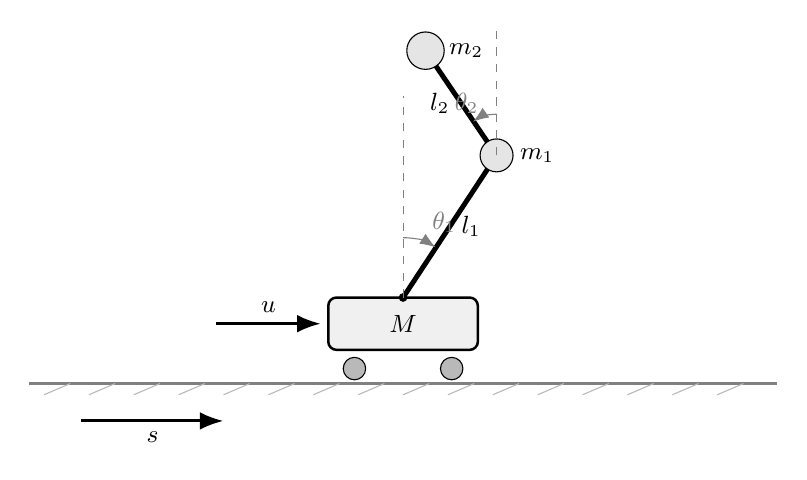
\begin{tikzpicture}[scale=0.95, every node/.style={font=\small}]
    \draw[gray, line width=1pt] (-5,-2.2) -- (5,-2.2);
    \foreach \x in {-4.8,-4.2,...,4.8} {
        \draw[gray!55] (\x,-2.35) -- (\x+0.35,-2.2);
    }

    \draw[fill=gray!12, draw=black, rounded corners=3pt, line width=0.9pt] (-1.0,-1.75) rectangle (1.0,-1.05);
    \draw[fill=gray!55, draw=black] (-0.65,-2.0) circle (0.15);
    \draw[fill=gray!55, draw=black] (0.65,-2.0) circle (0.15);
    \node at (0,-1.4) {$M$};

    \coordinate (P0) at (0,-1.05);
    \coordinate (P1) at (1.25,0.85);
    \coordinate (P2) at (0.30,2.25);

    \draw[black, line width=1.8pt] (P0) -- node[right] {$l_1$} (P1);
    \draw[black, line width=1.8pt] (P1) -- node[left] {$l_2$} (P2);
    \filldraw[fill=gray!20, draw=black] (P1) circle (0.22) node[right=5pt] {$m_1$};
    \filldraw[fill=gray!20, draw=black] (P2) circle (0.25) node[right=5pt] {$m_2$};
    \filldraw[fill=black] (P0) circle (0.05);

    \draw[gray, dashed] (P0) -- ++(0,2.7);
    \draw[gray, dashed] (P1) -- ++(0,1.7);
    \draw[-{Latex[length=2mm]}, gray] ($(P0)+(0,0.8)$) arc[start angle=90,end angle=57,radius=0.8];
    \node[gray] at (0.55,-0.05) {$\theta_1$};
    \draw[-{Latex[length=2mm]}, gray] ($(P1)+(0,0.55)$) arc[start angle=90,end angle=125,radius=0.55];
    \node[gray] at (0.85,1.55) {$\theta_2$};

    \draw[-{Latex[length=3mm]}, black, line width=1.1pt] (-2.5,-1.4) -- (-1.1,-1.4) node[midway, above] {$u$};
    \draw[-{Latex[length=3mm]}, black, line width=1.1pt] (-4.3,-2.7) -- (-2.4,-2.7) node[midway, below] {$s$};
\end{tikzpicture}
\caption{Cart with serial double pendulum and the variables used by the MATLAB model.}
\end{figure}

\begin{center}
\begin{tabular}{L{0.19\textwidth} L{0.50\textwidth} L{0.22\textwidth}}
\toprule
\textbf{Symbol} & \textbf{Meaning} & \textbf{Typical value in simulations} \\
\midrule
$s$ & Horizontal cart position & State component $x(1)$ \\
$\theta_1,\theta_2$ & Pendulum angles measured from upward vertical & State components $x(2),x(3)$ \\
$M$ & Cart mass & $1.0$ kg \\
$m_1,m_2$ & Point masses at the end of the first and second links & $0.20$ kg, $0.15$ kg \\
$l_1,l_2$ & Link lengths & $0.50$ m, $0.40$ m \\
$g$ & Gravitational acceleration & $9.81$ m/s$^2$ \\
$u$ & Horizontal force applied to the cart & Control input \\
\bottomrule
\end{tabular}
\end{center}

\subsection{Euler--Lagrange Modeling}

The MATLAB model is implemented in \texttt{underactuated\_model.m}. The position of the cart is $(s,0)$. The position of the first bob is
\begin{equation}
    p_1 =
    \begin{bmatrix}
        s + l_1\sin\theta_1 \\
        l_1\cos\theta_1
    \end{bmatrix},
\end{equation}
and the position of the second bob is
\begin{equation}
    p_2 =
    \begin{bmatrix}
        s + l_1\sin\theta_1 + l_2\sin\theta_2 \\
        l_1\cos\theta_1 + l_2\cos\theta_2
    \end{bmatrix}.
\end{equation}
Differentiating these positions gives the bob velocities. The kinetic energy is then the sum of the cart kinetic energy and the translational kinetic energy of the two point masses:
\begin{equation}
    T =
    \frac{1}{2}M\dot{s}^{2}
    + \frac{1}{2}m_1\left(\dot{x}_1^2+\dot{y}_1^2\right)
    + \frac{1}{2}m_2\left(\dot{x}_2^2+\dot{y}_2^2\right).
\end{equation}
With gravity acting in the negative vertical direction, the potential energy is
\begin{equation}
    V = (m_1+m_2)gl_1\cos\theta_1 + m_2gl_2\cos\theta_2.
\end{equation}
The Lagrangian is $L=T-V$. Applying the Euler--Lagrange equations gives the manipulator equation
\begin{equation}
    M(q)\ddot{q} + C(q,\dot{q})\dot{q} + G(q) = Bu.
\end{equation}
The input matrix is
\begin{equation}
    B =
    \begin{bmatrix}
        1 & 0 & 0
    \end{bmatrix}^{T},
\end{equation}
which means that the cart coordinate is directly actuated while the two angular coordinates are not. This rank-deficient actuation structure is the defining feature of the project.

The MATLAB function computes $M(q)$, $C(q,\dot{q})$, $G(q)$, and $B$ at each integration step. It then solves
\begin{equation}
    \ddot{q} = M(q)^{-1}\left(Bu-C(q,\dot{q})\dot{q}-G(q)-F_{\mathrm{fric}}\right),
\end{equation}
where optional viscous friction is included as
\begin{equation}
    F_{\mathrm{fric}} =
    \begin{bmatrix}
        b_{\mathrm{cart}} & b_{\mathrm{pend1}} & b_{\mathrm{pend2}}
    \end{bmatrix}^{T}
    \odot \dot{q}.
\end{equation}
Finally, the state derivative returned to \texttt{ode45} is
\begin{equation}
    \dot{x} =
    \begin{bmatrix}
        \dot{q} \\
        \ddot{q}
    \end{bmatrix}.
\end{equation}

\subsection{Model Analysis and Verification}

The script \texttt{simulation.m} performs several checks that are useful for detecting modeling errors. The first check is energy conservation. If $u=0$ and all friction terms are set to zero, the total mechanical energy $E=T+V$ should remain constant along the simulated trajectory. In numerical simulation there will usually be a small residual drift because of integration tolerances, but the drift should remain small when tight tolerances are used. This check is especially valuable because sign errors in the gravity vector or velocity coupling terms often show up immediately as artificial energy gain or loss.

The second check evaluates the dynamics at the two natural equilibrium configurations. With zero velocity and zero input, both the upright-upright configuration and the hanging-hanging configuration should produce zero acceleration. In the state convention used here, these states are
\begin{equation}
    x_{\mathrm{up}} =
    \begin{bmatrix}
        0&0&0&0&0&0
    \end{bmatrix}^{T},
    \qquad
    x_{\mathrm{down}} =
    \begin{bmatrix}
        0&\pi&\pi&0&0&0
    \end{bmatrix}^{T}.
\end{equation}
The script evaluates \texttt{underactuated\_model.m} at both states and prints the resulting derivative.

The third check compares numerical and analytic linearizations. Numerical linearization is computed by finite differences around an equilibrium. The analytic linearization is obtained from the manipulator equation. At an equilibrium with $\dot{q}=0$, the velocity-dependent terms vanish, so the local acceleration dynamics depend mainly on the mass matrix and the derivative of the gravity vector. The linear state-space model has the form
\begin{equation}
    \delta\dot{x} = A\delta x + B_{\ell}\delta u.
\end{equation}
The script reports the Frobenius norm of the difference between the numerical and analytic $A$ matrices. It also computes eigenvalues and checks the controllability rank using \texttt{rank(ctrb(A,B))}. For this six-state model, full controllability corresponds to rank 6.

\begin{center}
\begin{tabular}{L{0.22\textwidth} L{0.36\textwidth} L{0.32\textwidth}}
\toprule
\textbf{Verification step} & \textbf{Purpose} & \textbf{MATLAB implementation} \\
\midrule
Energy conservation & Confirms physically consistent dynamics in the unforced and frictionless case. & \texttt{simulation.m} computes $E=T+V$ and prints the maximum absolute and relative drift. \\
Equilibrium check & Confirms that exact upright and hanging configurations are stationary when velocities and input are zero. & \texttt{underactuated\_model.m} is evaluated at $x_{\mathrm{up}}$ and $x_{\mathrm{down}}$. \\
Linearization comparison & Detects algebraic mistakes in the dynamic equations and verifies local model consistency. & Numerical finite differences are compared with analytic linearization formulas. \\
Controllability test & Determines whether the local linearized model can be controlled through the cart force. & The rank of the controllability matrix is checked and expected to be 6. \\
\bottomrule
\end{tabular}
\end{center}

\sectionpage
\section{Controller Design}

\subsection{Local LQR Stabilizer}

The first controller is implemented in \texttt{control1.m}. It is designed for local stabilization around the upright equilibrium, where
\begin{equation}
    x^\ast = 0,
    \qquad
    u^\ast = 0.
\end{equation}
The nonlinear dynamics are numerically linearized around this equilibrium:
\begin{equation}
    \delta\dot{x} = A\delta x + B_{\ell}\delta u.
\end{equation}
The finite-difference step used in the code is $h=10^{-6}$. This provides a practical approximation of the Jacobian without requiring symbolic differentiation.

The LQR controller minimizes the quadratic cost
\begin{equation}
    J = \int_0^\infty \left(x^TQx + u^TRu\right)\,dt.
\end{equation}
The project uses
\begin{equation}
    Q = \mathrm{diag}\left(10,100,100,1,10,10\right),
    \qquad
    R=1.
\end{equation}
The large weights on the angular positions and angular velocities reflect the goal of balancing the pendulum links near the upright equilibrium. The smaller weight on cart position allows the controller to move the cart when necessary, while still discouraging excessive drift. MATLAB computes the feedback gain using \texttt{lqr(A,B,Q,R)}, and the control law is
\begin{equation}
    u = -Kx.
\end{equation}

The gain $K$ is stored in persistent variables inside \texttt{control1.m}. This is an efficient implementation choice because the gain depends only on the physical parameter struct. Recomputing the Riccati solution at every ODE evaluation would be unnecessary and would slow down the simulation. The gain is recomputed only when the parameter struct changes.

The stability interpretation of this controller is local. If the linearized closed-loop matrix $A-B_{\ell}K$ is stable, then the nonlinear closed-loop system is expected to be stable in a neighborhood of the upright equilibrium. However, the controller does not solve the global swing-up problem. If the pendulum starts near the hanging configuration, the linear approximation around upright is not valid, and the feedback law is not designed to inject the large amount of energy needed to raise the links.

\subsection{Energy-Shaping Swing-Up Controller}

The second controller is implemented in \texttt{control2.m}. It is designed to move the system from a large-angle configuration toward the upright equilibrium. The main idea is to compare the current total mechanical energy $E$ with the desired upright energy $E_{\mathrm{des}}$. If the system has too little energy, the controller should add energy. If it has too much energy, the controller should remove energy. Since the force can only act through the cart, the control input must exploit the coupling between cart acceleration and pendulum motion.

The total energy used in the controller is the same physical quantity used in the model verification:
\begin{equation}
    E = T+V.
\end{equation}
At the upright equilibrium the kinetic energy is zero and $\cos\theta_1=\cos\theta_2=1$, giving
\begin{equation}
    E_{\mathrm{des}} = (m_1+m_2)gl_1 + m_2gl_2.
\end{equation}
The control law implemented in \texttt{control2.m} is
\begin{equation}
    u =
    k(E-E_{\mathrm{des}})
    \operatorname{sign}\left(
        \dot{\theta}_1\cos\theta_1
        + \dot{\theta}_2\cos\theta_2
    \right),
\end{equation}
with $k=5$. The sign term approximates whether the pendulum masses are moving in a direction that can be used to raise or lower their potential energy. A fallback value of $1$ is used when the sign expression is zero, which prevents the controller from becoming stuck at exactly zero direction.

The controller also includes force saturation:
\begin{equation}
    -100\ \mathrm{N} \leq u \leq 100\ \mathrm{N}.
\end{equation}
This is not only physically reasonable but also numerically useful. Without saturation, the energy error can produce very large forces, which may lead to unrealistic motion or make the ODE integration unnecessarily difficult.

\subsection{Switching Logic and Hybrid Control Interpretation}

The energy-shaping controller is not intended to perform the final balancing task alone. Instead, it hands off to the local LQR controller when the system is close enough to upright. In the code, both angles are first wrapped to the interval $[-\pi,\pi]$. The hand-off condition is
\begin{equation}
    |\mathrm{wrap}(\theta_1)| < 0.2,\qquad
    |\mathrm{wrap}(\theta_2)| < 0.2,
\end{equation}
and
\begin{equation}
    |\dot{\theta}_1| < 1.0,\qquad
    |\dot{\theta}_2| < 1.0.
\end{equation}
When these conditions are satisfied, \texttt{control2.m} calls \texttt{control1.m} and returns the LQR input. This makes the complete controller a hybrid controller: one mode performs energy shaping and the other mode performs local stabilization.

This hybrid structure is appropriate for the problem because the swing-up and balancing tasks are qualitatively different. Swing-up requires large nonlinear motion and energy transfer. Balancing requires precise local feedback around an unstable equilibrium. Combining the two methods gives a controller that is more capable than either component alone.

\sectionpage
\section{Simulation Results}

\subsection{Simulation Environment}

The project uses MATLAB's \texttt{ode45} solver to integrate the nonlinear state equations. The model function accepts either a scalar input or a function handle for feedback control. This makes the same dynamics file usable for open-loop verification, local LQR control, and nonlinear swing-up control.

The controller simulations use the following nominal parameters:
\begin{center}
\begin{tabular}{L{0.25\textwidth} L{0.28\textwidth} L{0.32\textwidth}}
\toprule
\textbf{Parameter} & \textbf{Value} & \textbf{Description} \\
\midrule
$M$ & $1.0$ kg & Cart mass \\
$m_1$ & $0.20$ kg & First pendulum point mass \\
$m_2$ & $0.15$ kg & Second pendulum point mass \\
$l_1$ & $0.50$ m & First link length \\
$l_2$ & $0.40$ m & Second link length \\
$g$ & $9.81$ m/s$^2$ & Gravitational acceleration \\
$b_{\mathrm{cart}}$ & $0.05$ N s/m & Cart viscous friction for controller simulations \\
$b_{\mathrm{pend1}}$ & $0.001$ N m s/rad & First joint viscous friction \\
$b_{\mathrm{pend2}}$ & $0.001$ N m s/rad & Second joint viscous friction \\
\bottomrule
\end{tabular}
\end{center}

The verification script uses a separate friction-free parameter set when checking energy conservation. This is important because energy should not be conserved when friction is present. The controller scripts use light damping to make the simulations more realistic and numerically well behaved.

\subsection{Model Verification Simulation}

The script \texttt{simulation.m} first tests the unforced, frictionless response from
\begin{equation}
    x_0 =
    \begin{bmatrix}
        0 & \pi-0.30 & \pi+0.20 & 0 & 0 & 0
    \end{bmatrix}^{T}.
\end{equation}
It integrates the model for 10 seconds and computes the total mechanical energy at every time sample. The expected result is that the energy drift remains close to zero. The script then plots the state trajectories and the energy drift. These plots are useful because they show both the qualitative pendulum motion and the quantitative conservation behavior.

The same script then evaluates the upright and hanging equilibria, computes numerical and analytic linearizations, prints eigenvalues, and checks controllability. The controllability result is especially relevant for the LQR design: if the linearized upright model were not controllable, then no full-state feedback law could arbitrarily assign the local closed-loop behavior.

\subsection{Local LQR Simulation}

The script \texttt{controller1\_sim.m} tests the local LQR controller from the initial condition
\begin{equation}
    x_0 =
    \begin{bmatrix}
        0 & 0.15 & -0.15 & 0 & 0 & 0
    \end{bmatrix}^{T}.
\end{equation}
This state is close to the upright equilibrium, so it lies in the intended operating region of the linear controller. The simulation runs for 6 seconds. The script plots the cart position, both pendulum angles, all three velocities, and the control input $u$.

The expected behavior is that $\theta_1$ and $\theta_2$ decay toward zero, while the cart moves as needed to create stabilizing acceleration. The control signal should remain bounded, and the final angle errors printed by the script should be small. If the initial angles were made much larger, the LQR controller would no longer be expected to perform well because the linear approximation would no longer describe the nonlinear plant accurately.

\subsection{Swing-Up and Capture Simulation}

The script \texttt{controller2\_sim.m} tests the energy-shaping controller from an initial condition near hanging:
\begin{equation}
    x_0 =
    \begin{bmatrix}
        0 & \pi-0.1 & \pi+0.1 & 0 & 0 & 0
    \end{bmatrix}^{T}.
\end{equation}
The simulation runs for 30 seconds. In addition to state and control plots, the script computes the total mechanical energy and plots it together with the desired upright energy $E_{\mathrm{des}}$.

The expected response has two phases. In the first phase, the energy-shaping controller pumps energy into the system and causes large pendulum motion. The total energy should move toward the desired upright energy level, although it may oscillate because the system is nonlinear and the control input is saturated. In the second phase, when the angles and angular velocities are sufficiently close to upright, the controller switches to LQR. After the switch, the state should converge toward the upright equilibrium.

\begin{longtable}{L{0.18\textwidth} L{0.23\textwidth} L{0.28\textwidth} L{0.21\textwidth}}
\toprule
\textbf{Script} & \textbf{Initial condition} & \textbf{Purpose} & \textbf{Main outputs} \\
\midrule
\endfirsthead
\toprule
\textbf{Script} & \textbf{Initial condition} & \textbf{Purpose} & \textbf{Main outputs} \\
\midrule
\endhead
\texttt{simulation.m} & Near hanging for free response; exact upright and hanging states for equilibrium checks. & Validates the physical model through energy conservation, equilibrium checks, linearization comparison, and controllability. & State plots, energy drift, eigenvalues, controllability rank, animation. \\
\texttt{controller1\_sim.m} & $[0,0.15,-0.15,0,0,0]^T$ & Demonstrates local LQR balance from a small perturbation near upright. & States, velocities, control force, final angle errors, peak $|u|$. \\
\texttt{controller2\_sim.m} & $[0,\pi-0.1,\pi+0.1,0,0,0]^T$ & Demonstrates nonlinear swing-up and transition to local LQR stabilization. & States, velocities, control force, total energy, desired energy, final wrapped angle errors. \\
\bottomrule
\end{longtable}

For a final submitted report, the MATLAB figures generated by these scripts should be exported and inserted into this section. The most important plots are the angle trajectories, the control input, and the total energy curve for the swing-up controller. These figures would directly show whether the LQR controller stabilizes the upright equilibrium and whether the energy-shaping controller reaches the LQR capture region.

\sectionpage
\section{Conclusions}

The MATLAB project implements a complete modeling and control workflow for an underactuated cart double-pendulum. The Euler--Lagrange model is expressed in manipulator form, which makes the physical structure clear and supports both simulation and linearization. The verification script checks important properties of the model, including energy conservation, equilibrium behavior, agreement between numerical and analytic linearization, and controllability of the local linearized models.

The controller design illustrates why underactuated systems often require more than one control idea. The LQR controller is suitable for local stabilization near the upright equilibrium and provides a systematic way to trade off state regulation against input effort. However, because it is based on a local linearization, it is not a global swing-up controller. The energy-shaping controller addresses the larger motion problem by regulating total mechanical energy and then transferring control to the LQR once the state is close enough to upright.

The main limitation of the current project is that the swing-up controller is heuristic. It uses a simple energy-pumping law, fixed gains, saturation, and a hand-selected switching condition. These choices are reasonable for simulation, but they do not by themselves provide a complete proof of global convergence or robustness. Further work could include systematic gain tuning, actuator constraint analysis, switching hysteresis, robustness tests under parameter uncertainty, and exported simulation figures comparing performance across initial conditions.

Overall, the project demonstrates the central challenge of underactuated robotics: the controller must use nonlinear dynamic coupling to influence passive coordinates. The combination of Euler--Lagrange modeling, local linear analysis, LQR stabilization, and nonlinear energy shaping provides a strong foundation for a more detailed experimental or theoretical study.

\sectionpage
\begin{thebibliography}{9}
\bibitem{xu2008}
R. Xu and U. Ozguner, ``Sliding mode control of a class of underactuated systems,'' \emph{Automatica}, vol. 44, no. 1, pp. 233--241, 2008.
\end{thebibliography}

\sectionpage
\appendix
\section{Model Matrices and MATLAB File Roles}

This appendix records the implementation details that support the main text. Let
\[
s_1=\sin\theta_1,\quad
c_1=\cos\theta_1,\quad
s_2=\sin\theta_2,\quad
c_2=\cos\theta_2,
\]
and
\[
s_{12}=\sin(\theta_1-\theta_2),\quad
c_{12}=\cos(\theta_1-\theta_2).
\]
The mass matrix implemented in \texttt{underactuated\_model.m} is
\begin{equation}
M(q)=
\begin{bmatrix}
M+m_1+m_2 & (m_1+m_2)l_1c_1 & m_2l_2c_2 \\
(m_1+m_2)l_1c_1 & (m_1+m_2)l_1^2 & m_2l_1l_2c_{12} \\
m_2l_2c_2 & m_2l_1l_2c_{12} & m_2l_2^2
\end{bmatrix}.
\end{equation}
The Coriolis and centrifugal matrix is
\begin{equation}
C(q,\dot{q})=
\begin{bmatrix}
0 & -(m_1+m_2)l_1s_1\dot{\theta}_1 & -m_2l_2s_2\dot{\theta}_2 \\
0 & 0 & m_2l_1l_2s_{12}\dot{\theta}_2 \\
0 & -m_2l_1l_2s_{12}\dot{\theta}_1 & 0
\end{bmatrix}.
\end{equation}
The gravity vector and input vector are
\begin{equation}
G(q)=
\begin{bmatrix}
0 \\
-(m_1+m_2)gl_1\sin\theta_1 \\
-m_2gl_2\sin\theta_2
\end{bmatrix},
\qquad
B=
\begin{bmatrix}
1\\0\\0
\end{bmatrix}.
\end{equation}

\begin{center}
\begin{tabular}{L{0.28\textwidth} L{0.62\textwidth}}
\toprule
\textbf{File} & \textbf{Role in the project} \\
\midrule
\texttt{underactuated\_model.m} & Defines the nonlinear state derivative and the manipulator matrices used by all simulations. \\
\texttt{simulation.m} & Runs the model verification tests: energy conservation, equilibrium checks, linearization comparison, controllability, and animation. \\
\texttt{control1.m} & Constructs and applies the cached LQR stabilizer around the upright equilibrium. \\
\texttt{control2.m} & Implements energy shaping for swing-up and switches to \texttt{control1.m} near upright. \\
\texttt{controller1\_sim.m} & Simulates local LQR balancing from a small upright perturbation. \\
\texttt{controller2\_sim.m} & Simulates swing-up from near hanging followed by LQR capture. \\
\texttt{animate\_cartpole.m} & Provides real-time visualization of the cart and double-pendulum trajectory. \\
\bottomrule
\end{tabular}
\end{center}

\end{document}
